% ----------------------------------------------------------------
% AMS-LaTeX Paper ************************************************
% **** -----------------------------------------------------------
%\documentclass{amsart}
%\usepackage{txfonts}
%\documentclass[12pt,oneside]{article}
\documentclass{amsart}
\usepackage{graphicx}
\usepackage{enumitem}
% ----------------------------------------------------------------
\vfuzz2pt % Don't report over-full v-boxes if over-edge is small
\hfuzz2pt % Don't report over-full h-boxes if over-edge is small
% THEOREMS -------------------------------------------------------
\newtheorem{thm}{Theorem}[section]
\newtheorem{cor}[thm]{Corollary}
\newtheorem{lem}[thm]{Lemma}
\newtheorem{prop}[thm]{Proposition}
\theoremstyle{definition}
\newtheorem{defn}[thm]{Definition}
\theoremstyle{Exercise}
\newtheorem{ex}[thm]{Exercise}
\theoremstyle{remark}
\newtheorem{rem}[thm]{Remark}
\theoremstyle{rule}
\newtheorem{rul}[thm]{Rule}

\numberwithin{equation}{section}
% MATH -----------------------------------------------------------
\newcommand{\norm}[1]{\left\Vert#1\right\Vert}
\newcommand{\abs}[1]{\left\vert#1\right\vert}
\newcommand{\set}[1]{\left\{#1\right\}}
\newcommand{\Real}{\mathbb{R}}
\newcommand{\Z}{\mathbb{Z}}
\newcommand{\To}{\longrightarrow}
\newcommand{\BX}{\bB(X)}
\newcommand{\A}{\mathcal{A}}
% ----------------------------------------------------------------

% define some simple, commonly-used commands
\newcommand{\eps}{\varepsilon}
\newcommand{\dsum}{\displaystyle\sum}
\newcommand{\dint}{\displaystyle\int}

\newcommand{\pdr}[2]{\dfrac{\partial{#1}}{\partial{#2}}}
\newcommand{\pdrr}[2]{\dfrac{\partial^2{#1}}{\partial{#2}^2}}
\newcommand{\pdrt}[3]{\dfrac{\partial^2{#1}}{\partial{#2}{\partial{#3}}}}
\newcommand{\dr}[2]{\dfrac{d{#1}}{d{#2}}}
\newcommand{\aver}[1]{\langle {#1} \rangle}
\newcommand{\Baver}[1]{\Big\langle {#1} \Big\rangle}

\newcommand{\bzero}{\mathbf{0}}
\newcommand{\bGamma}{\mbox{\boldmath{$\Gamma$}}}
\newcommand{\btheta}{\boldsymbol \theta}
\newcommand{\bchi}{\mbox{\boldmath{$\chi$}}}
\newcommand{\bnu}{\boldsymbol \nu}
\newcommand{\bmu}{\boldsymbol \mu}
\newcommand{\brho}{\mbox{\boldmath{$\rho$}}}
\newcommand{\bxi}{\boldsymbol \xi}
\newcommand{\bnabla}{\boldsymbol \nabla}
\newcommand{\bOm}{\boldsymbol \Omega}
\newcommand{\blambda}{\boldsymbol \lambda}
\newcommand{\bsigma}{\boldsymbol \sigma}

\newcommand{\bbR}{\mathbb{R}}
\newcommand{\bbC}{\mathbb{C}}
\newcommand{\bbQ}{\mathbb{Q}}
\newcommand{\bbN}{\mathbb{N}}
\newcommand{\bbZ}{\mathbb{Z}}

\newcommand{\ba}{\mathbf{a}}
\newcommand{\bb}{\mathbf{b}}
\newcommand{\bc}{\mathbf{c}}
\newcommand{\bd}{\mathbf{d}}
\newcommand{\be}{\mathbf{e}}
\newcommand{\bff}{\mathbf{f}}
\newcommand{\bg}{\mathbf{g}}
\newcommand{\bh}{\mathbf{h}}
\newcommand{\bi}{\mathbf{i}}
\newcommand{\bj}{\mathbf{j}}
\newcommand{\bk}{\mathbf{k}}
\newcommand{\bl}{\mathbf{l}}
\newcommand{\bm}{\mathbf{m}}
\newcommand{\bn}{\mathbf{n}}
\newcommand{\bo}{\mathbf{o}}
\newcommand{\bp}{\mathbf{p}}
\newcommand{\bq}{\mathbf{q}}
\newcommand{\br}{\mathbf{r}}
\newcommand{\bs}{\mathbf{s}}
\newcommand{\bt}{\mathbf{t}}
\newcommand{\bu}{\mathbf{u}}
\newcommand{\bv}{\mathbf{v}}
\newcommand{\bw}{\mathbf{w}}
\newcommand{\bx}{\mathbf{x}}
\newcommand{\by}{\mathbf{y}}
\newcommand{\bz}{\mathbf{z}}
\newcommand{\bA}{\mathbf{A}}
\newcommand{\bB}{\mathbf{B}}
\newcommand{\bC}{\mathbf{C}}
\newcommand{\bD}{\mathbf{D}}
\newcommand{\bE}{\mathbf{E}}
\newcommand{\bF}{\mathbf{F}}
\newcommand{\bG}{\mathbf{G}}
\newcommand{\bH}{\mathbf{H}}
\newcommand{\bI}{\mathbf{I}}
\newcommand{\bJ}{\mathbf{J}}
\newcommand{\bK}{\mathbf{K}}
\newcommand{\bL}{\mathbf{L}}
\newcommand{\bM}{\mathbf{M}}
\newcommand{\bN}{\mathbf{N}}
\newcommand{\bO}{\mathbf{O}}
\newcommand{\bP}{\mathbf{P}}
\newcommand{\bQ}{\mathbf{Q}}
\newcommand{\bR}{\mathbf{R}}
\newcommand{\bS}{\mathbf{S}}
\newcommand{\bT}{\mathbf{T}}
\newcommand{\bU}{\mathbf{U}}
\newcommand{\bV}{\mathbf{V}}
\newcommand{\bW}{\mathbf{W}}
\newcommand{\bX}{\mathbf{X}}
\newcommand{\bY}{\mathbf{Y}}
\newcommand{\bZ}{\mathbf{Z}}

\newcommand{\cA}{\mathcal{A}}
\newcommand{\cB}{\mathcal{B}}
\newcommand{\cC}{\mathcal{C}}
\newcommand{\cD}{\mathcal{D}}
\newcommand{\cE}{\mathcal{E}}
\newcommand{\cF}{\mathcal{F}}
\newcommand{\cG}{\mathcal{G}}
\newcommand{\cH}{\mathcal{H}}
\newcommand{\cI}{\mathcal{I}}
\newcommand{\cJ}{\mathcal{J}}
\newcommand{\cK}{\mathcal{K}}
\newcommand{\cL}{\mathcal{L}}
\newcommand{\cM}{\mathcal{M}}
\newcommand{\cN}{\mathcal{N}}
\newcommand{\cO}{\mathcal{O}}
\newcommand{\cP}{\mathcal{P}}
\newcommand{\cQ}{\mathcal{Q}}
\newcommand{\cR}{\mathcal{R}}
\newcommand{\cS}{\mathcal{S}}
\newcommand{\cT}{\mathcal{T}}
\newcommand{\cU}{\mathcal{U}}
\newcommand{\cV}{\mathcal{V}}
\newcommand{\cW}{\mathcal{W}}
\newcommand{\cX}{\mathcal{X}}
\newcommand{\cY}{\mathcal{Y}}
\newcommand{\cZ}{\mathcal{Z}}

%%%%%%%%%%%%%%Start%%%%%%%%%%%%%Start%%%%%%%%%%%Start%%%%%%%%%%%%%%%Start%%%%%%%%%%%%%%%%%%%%%%%%%Start%%%%%%%%%%%%%%%%
%%%%%%%%%%%%%%Start%%%%%%%%%%%%%Start%%%%%%%%%%%Start%%%%%%%%%%%%%%%Start%%%%%%%%%%%%%%%%%%%%%%%%%Start%%%%%%%%%%%%%%%%
%%%%%%%%%%%%%%Start%%%%%%%%%%%%%Start%%%%%%%%%%%Start%%%%%%%%%%%%%%%Start%%%%%%%%%%%%%%%%%%%%%%%%%Start%%%%%%%%%%%%%%%%
%\documentclass[12pt,oneside]{article}

\usepackage{pdfpages}
%--------------
\usepackage{enumitem}
%-------------Tasks
%\usepackage{tasks} %\begin{tasks} \item \end{tasks}
%\bfseries Horizontal list: a = alphabetical \normalfont
%\begin{tasks}[counter-format = {tsk[a].},label-offset = {0.6em},label-format = {\bfseries}](6)
%\task One
%\task Two
%\task Three
%\task Four
%\task Five
%\task Six
%\task Seven
%\task Eight
%\task Nine
%\task Ten
%\end{tasks}
%\vglue5mm
%\bfseries Horizontal list: A = Alphabetical \normalfont
%\begin{tasks}[counter-format = {(tsk[A])},label-offset = {0.8em},label-format = {\bfseries}](3)
%\task One
%\task Two
%\task Three
%\task Four
%\task Five
%\task Six
%\task Seven
%\task Eight
%\task Nine
%\task Ten
%\end{tasks}

%___________________________
\usepackage[margin=2.5cm]{geometry}

\geometry{hmargin=3cm, vmargin=2cm}
\usepackage{tikz}
\def\width{18}
\def\hauteur{13}

\pagestyle{plain}

%%%%%%%%%%%%%%Start%%%%%%%%%%%%%Start%%%%%%%%%%%Start%%%%%%%%%%%%%%%Start%%%%%%%%%%%%%%%%%%%%%%%%%Start%%%%%%%%%%%%%%%%
%%%%%%%%%%%%%%Start%%%%%%%%%%%%%Start%%%%%%%%%%%Start%%%%%%%%%%%%%%%Start%%%%%%%%%%%%%%%%%%%%%%%%%Start%%%%%%%%%%%%%%%%
%%%%%%%%%%%%%%Start%%%%%%%%%%%%%Start%%%%%%%%%%%Start%%%%%%%%%%%%%%%Start%%%%%%%%%%%%%%%%%%%%%%%%%Start%%%%%%%%%%%%%%%%

\usepackage{fancyhdr}

\pagestyle{fancy}
\fancyhf{}
\rhead{}
\chead{\includegraphics[scale=.1]{snhu_logo.png}}
\begin{document}
	\title{\sf MAT 230 Exam Two}%

	%\thm{bbjh}

	\begin{center}
		\includegraphics[scale=.1]{snhu_logo.png}
	\end{center}

	%\thm{bbjh}
	\maketitle
	This document is proprietary to Southern New Hampshire University. It and the
	problems within may not be posted on any non-SNHU website.\\\\\\\\
	\begin{center}
		%Enter your name below this line:
		Ryan Hatch
	\end{center}

	\begin{center}
		\rule{\textwidth}{0.4pt}
	\end{center}
	\newpage
	\section*{}
	\section*{}
	Directions: Type your solutions into this document and be sure to show all steps
	for arriving at your solution. Just giving a final number may not receive full
	credit. \\
	\section*{Problem 1}
	\noindent
	This question has 2 parts.
	\subsection*{Part 1:}
	Suppose that $F$ and $X$ are events from a common sample space with
	$P(F) \neq 0$ and $P(X) \neq 0$. \\
	\begin{enumerate}[label=(\alph{*})]
		\item Prove that $P(X) = P(X|F)P(F) + P(X|\bar{F})P(\bar{F})$. Hint: Explain
			why $P(X|F)P(F) = P(X \cap F)$ is another way of writing the definition of
			conditional probability, and then use that with the logic from the proof
			of Theorem 4.1.1. \\\\
			%Enter your answer below this comment line.
			Considering that $P(X|F) = \frac{P(X \cap F)}{P(F)}$. Means, $P(X \cap F) =
			P(X|F)P(F)$.

			Next, the sample space was then partitioned into the event: $F$ and its complement
			$\bar{F}$. thus, the event $X$ can occur either with $F$ or with $\bar{F}$,
			and these two cases are mutually exclusive.

			Next, by the Law of Total Probability, I noted that $P(X)$ can be obtained
			by adding $P(X)$ occurring with $F$ and $P(X)$ occurring with $\bar{F}$: $P
			(X) = P(X \cap F) + P(X \cap \bar{F})$.

			Now, I used the same technique that I used previously to express
			$P(X \cap \bar{F})$ in terms of conditional probability: $P(X \cap \bar{F})
			= P(X|\bar{F})P(\bar{F})$.

			Combining the previous expression into the Law of Total Probability, I got:
			$P(X) = P(X|F)P(F) + P(X|\bar{F})P(\bar{F})$. \\\\

		\item Explain why $P(F|X) = P(X|F)P(F)/P(X)$ is another way of stating Theorem
			4.2.1 Bayes’ Theorem. \\\\
			%Enter your answer below this comment line.
			From the definition of Conditional Probability, I know that $P(F|X) = \frac{P(F
			\cap X)}{P(X)}$.\\ Next I noted that $P(F \cap X) = P(X \cap F)$, because
			the intersection is commutative. Then, I applied the definition of
			conditional probability again, to see that $P(X \cap F) = P(X|F)P(F)$.
			Then, I was able to substitute what I got earlier into the definition from
			the beginning, showing Bayes' Theorem: $P(F|X) = \frac{P(X|F)P(F)}{P(X)}$.
			\\\\
	\end{enumerate}
	\subsection*{Part 2:}
	A website reports that 70\% of its users are from outside a certain country. Out
	of their users from outside the country, 60\% of them log on every day. Out of
	their users from inside the country, 80\% of them log on every day. \\
	\begin{enumerate}[label=(\alph{*})]
		\item What percent of all users log on every day? Hint: Use the equation from
			Part 1 (a). \\\\
			%Enter your answer below this comment line.
			The percent of all users who log on every day can be calculated using the formula
			from Part 1 (a), which is the Law of Total Probability:
			\[
				P(\text{{login}}) = P(\text{{login}}| \text{{outside}})P(\text{{outside}}
				) + P(\text{{login}}| \text{{inside}})P(\text{{inside}})
			\]
			Given that:
			\[
				P(\text{{outside}}) = 0.70
			\]
			\[
				P(\text{{login}}| \text{{outside}}) = 0.60
			\]
			\[
				P(\text{{login}}| \text{{inside}}) = 0.80
			\]
			\[
				P(\text{{inside}}) = 1 - P(\text{{outside}}) = 0.30
			\]

			With this, the overall probability that a user logs on every day would be:
			\[
				P(\text{{login}}) = 0.60 \times 0.70 + 0.80 \times 0.30 = 0.66
			\]
			So, 66 percent of all users log on every day. \\\\

		\item Using Bayes’ Theorem, out of users who log on every day, what is the probability
			that they are from inside the country? \\\\
			%Enter your answer below this comment line.
			Using Bayes’ Theorem:
			\[
				P(\text{{inside}}| \text{{login}}) = \frac{P(\text{{login}} |
				\text{{inside}})P(\text{{inside}})}{P(\text{{login}})}
			\]
			Given my previous calculations, I got:
			\[
				P(\text{{inside}}| \text{{login}}) = \frac{0.80 \times 0.30}{0.66}\approx
				0.364
			\]
			So, there is approximately a 36.4 percent probability that users who log on
			every day are from inside the country. \\\\
	\end{enumerate}
	\newpage

	~\\
	\section*{Problem 2}
	\noindent
	This question has 2 parts.
	\subsection*{Part 1:}
	The drawing below shows a Hasse diagram for a partial order on the set: \\ $\{A
	, \;B,\; C,\; D,\; E,\; F,\; G,\; H,\; I, \; J\}$
	\begin{center}
		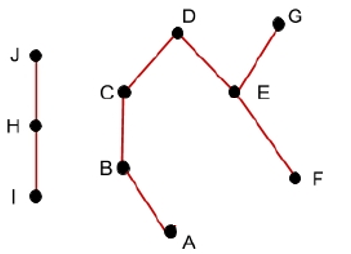
\includegraphics[width=2.5in]{NewHasse}
	\end{center}
	{\color{blue} {\bf Figure 1:} \emph{A Hasse diagram shows 10 vertices and 8 edges. The vertices, represented by dots, are as follows: vertex J is upward of vertex H; vertex H is upward of vertex I; vertex B is inclined upward to the left of vertex A; vertex C is upward of vertex B; vertex D is inclined upward to the right of vertex C; vertex E is inclined upward to the left of vertex F; vertex G is inclined upward to the right of vertex E. The edges, represented by line segments between the vertices are as follows: 3 vertical edges connect the following vertices: B and C, H and I, and H and J; 5 inclined edges connect the following vertices: A and B, C and D, D and E, E and F, and E and G. } }
	\\\\ Determine the properties of the Hasse diagram based on the following
	questions:

	\begin{enumerate}[label=(\alph{*})]
		\item What are the minimal elements of the partial order? \\\\
			%Enter your answer below this comment line.
			The \textbf{minimal elements} are those that have no edges descending to
			them. In this diagram, the minimal element is:
			\begin{itemize}
				\item \textbf{A}.
			\end{itemize}

		\item What are the maximal elements of the partial order? \\\\
			%Enter your answer below this comment line.
			The \textbf{maximal elements} are those with no edges ascending from them.
			Here, the maximal elements are:
			\begin{itemize}
				\item \textbf{J}, \textbf{D}, and \textbf{G}.
			\end{itemize}

		\item Which of the following pairs are comparable?
			\[
				(A,\, D),\; (J,\, F),\; (B,\, E),\; (G,\, F),\; (D,\, B),\; (C,\, F),\; (
				H,\, I), (C,\, E)
			\]
			\\\\
			%Enter your answer below this comment line.
			Two elements are \textbf{comparable} if you can travel from one to the
			other following the edges without backtracking. Based on this diagram:
			\begin{itemize}
				\item \textbf{A} and \textbf{B} are comparable because you can move upwards
					from \textbf{A} to \textbf{B}.

				\item \textbf{B} and \textbf{C} are comparable because you can move upwards
					from \textbf{B} to \textbf{C}.

				\item \textbf{C} and \textbf{D} are comparable because you can move upwards
					from \textbf{C} to \textbf{D}.

				\item \textbf{D} and \textbf{E} are not comparable; there's no way to
					move from \textbf{D} to \textbf{E} or vice versa following the edges.

				\item \textbf{E} and \textbf{F} are comparable because you can move downwards
					from \textbf{E} to \textbf{F}.

				\item \textbf{E} and \textbf{G} are comparable because you can move upwards
					from \textbf{E} to \textbf{G}.
			\end{itemize}
	\end{enumerate}
	\newpage
	~\\
	\subsection*{Part 2:}
	Consider the partial order with domain $\{3,\, 5,\, 6, \,7,\, 10,\, 14,\, 20,\,
	30,\, 60,\, 70\}$ and with $x\,\leq \,y$ if $x$ evenly divides $y$. Select the
	correct Hasse diagram for the partial order.

	\begin{enumerate}[label=(\alph{*})]
		\item \fbox{
			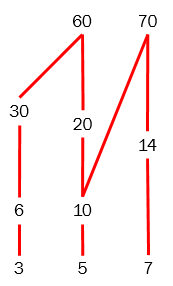
\includegraphics[height=3in]{Figure2}
			\\

			} \\\\
			{\color{blue}{\bf Figure 2:} \emph{A Hasse diagram shows a set of elements {3; 5; 6; 7; 10; 14; 20; 30; 60, 70}. There are lines connecting 3 and 6, 6 and 30, 30 and 60, 5 and 10, 10 and 20, 20 and 60, 10 and 70, 7 and 14, 14 and 70. } }
			\\ \\
			%Enter your answer below this comment line.
			\\\\
			\newpage
			~\\~\\

		\item \fbox{
			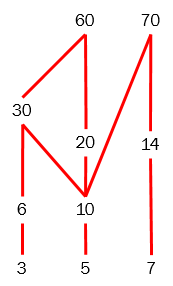
\includegraphics[height=3in]{Figure3}
			} \\\\
			{\color{blue}{\bf Figure 3:} \emph{A Hasse diagram shows a set of elements {3; 5; 6; 7; 10; 14; 20; 30; 60, 70}. There are lines connecting 3 and 6, 6 and 30, 30 and 60, 5 and 10, 10 and 30, 10 and 20, 20 and 60, 10 and 70, 7 and 14, 14 and 70. } }
			\\ \\
			%Enter your answer below this comment line.
			the correct Hasse diagram is described in \textbf{Figure 3}. This result
			resulted by comparing the explicit connections and relations depicted in
			the diagrams with the divisibility relations among the set elements.

			The connections in \textbf{Figure 3} showcase the necessary relations that
			define our partial order, such as:
			\begin{itemize}
				\item 3 dividing 6, 30, and indirectly 60 through 30,

				\item 5 dividing 10, 20, 30, and indirectly 60 and 70 through 10 and 30,

				\item 6 dividing 30 and indirectly 60 through 30,

				\item 7 dividing 14 and indirectly 70 through 14,

				\item 10 dividing 20, 30, and indirectly 60 and 70 through 20 and 30,

				\item 14 dividing 70,

				\item 20 dividing 60,

				\item 30 dividing 60.
			\end{itemize}
			These relations are best represented in \textbf{Figure 3}, making it the best
			representation of the partial order based on divisibility among the given set
			elements. \\\\
			\newpage
			~\\~\\

		\item \fbox{
			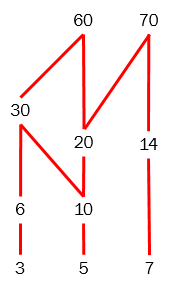
\includegraphics[height=3in]{Figure4}
			\\ } \\\\
			{\color{blue}{\bf Figure 4:} \emph{A Hasse diagram shows a set of elements {3; 5; 6; 7; 10; 14; 20; 30; 60, 70}. There are lines connecting 3 and 6, 6 and 30, 30 and 60, 5 and 10, 10 and 30, 10 and 20, 20 and 60, 20 and 70, 7 and 14, 14 and 70. } }
			\\ \\
			%Enter your answer below this comment line.
			\\\\
			\newpage
			~\\~\\

		\item \fbox{
			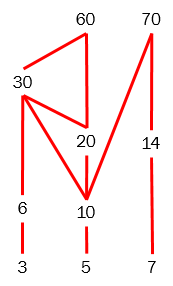
\includegraphics[height=3in]{Figure5}
			} \\\\
			{\color{blue}{\bf Figure 5:} \emph{A Hasse diagram shows a set of elements {3; 5; 6; 7; 10; 14; 20; 30; 60, 70}. There are lines connecting 3 and 6, 6 and 30, 30 and 60, 5 and 10, 10 and 30, 10 and 20, 20 and 30, 20 and 60, 10 and 70, 7 and 14, 14 and 70. } }
			\\\\
			%Enter your answer below this comment line.
			\\\\
	\end{enumerate}
	\newpage
	~\\
	\section*{Problem 3}
	A car dealership sells cars that were made in 2015 through 2020. Let the cars for
	sale be the domain of a relation R where two cars are related if they were made
	in the same year.

	\begin{enumerate}[label=(\alph{*})]
		\item Prove that this relation is an equivalence relation. \\\\
			%Enter your answer below this comment line.
			The relation $R$ is an equivalence relation because it satisfies the following
			properties: \begin{itemize}
			\begin{itemize}
				\item \textbf{Reflexivity}: Every car is related to itself since it is made
					in the same year as itself.

				\item \textbf{Symmetry}: If car $a$ is related to car $b$, then car $b$
					is related to car $a$ as they are made in the same year.

				\item \textbf{Transitivity}: If car $a$ is related to car $b$, and car
					$b$ is related to car $c$, then car $a$ is also related to car $c$, as
					they are all made in the same year.
			\end{itemize}

			Therefore, $R$ is an equivalence relation. \\\\

		\item Describe the partition defined by the equivalence classes. \\\\
			%Enter your answer below this comment line.
			The partition defined by the equivalence classes will consist of six sets,
			each containing cars from one of the years between 2015 and 2020. Each set,
			or equivalence class, can be represented as
			$[2015], [2016], [2017], [2018], [2019], [2020]$, where the cars in each class
			are all the cars made in that respective year. \\\\
	\end{enumerate}
	\newpage
	~\\
	\section*{Problem 4}
	Analyze each graph below to determine whether it has an Euler circuit and/or
	an Euler trail.
	\begin{itemize}
		\item If it has an Euler circuit, specify the nodes for one.

		\item If it does not have an Euler circuit, justify why it does not.

		\item If it has an Euler trail, specify the nodes for one.

		\item If it does not have an Euler trail, justify why it does not.
	\end{itemize}
	\begin{enumerate}[label=(\alph{*})]
		\item \fbox{
			
\includegraphics[width=4in]{Figure6}
			} \\\\
			{\color{blue} {\bf Figure 6:} \emph{An undirected graph has 6 vertices, a through f. There are 8-line segments that are between the following vertices: a and b, a and c, a and d, a and f, b and c, b and e, b and f, d and e. } }\\\\
			%Enter your answer below this comment line.
			All vertices have an even degree. Therefore, it has an Euler circuit. An example
			of an Euler circuit in this graph starting at vertex 'a' could be:
			$a \rightarrow b \rightarrow c \rightarrow a \rightarrow d \rightarrow e \rightarrow
			b \rightarrow f \rightarrow a$. \\\\
			\newpage
			~\\~\\

		\item \fbox{
			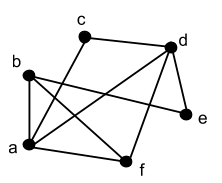
\includegraphics[width=4in]{Figure7}
			} \\\\
			{\color{blue} {\bf Figure 7:} \emph{ An undirected graph has 6 vertices, a through f. There are 9-line segments that are between the following vertices: a and b, a and c, a and d, a and f, b and e, b and f, c and d, d and e, d and f. } }
			\\\\
			%Enter your answer below this comment line.
			All vertices have an even degree except vertices 'a' and 'd', which have
			an odd degree.

			With this said, it does not have an Euler circuit but has an Euler trail.
			An example of an Euler trail in this graph could be: $a \rightarrow b \rightarrow
			f \rightarrow a \rightarrow c \rightarrow d \rightarrow e \rightarrow b \rightarrow
			e \rightarrow d$. \\\\
			\newpage
			~\\~\\

		\item \fbox{
			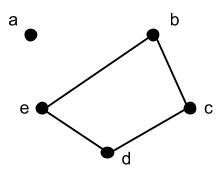
\includegraphics[width=4in]{Figure8}
			} \\\\
			{\color{blue} {\bf Figure 8: } \emph{An undirected graph has 5 vertices, a through e. There are 4-line segments that are between the following vertices: b and c, b and e, c and d, d and e. } }
			\\\\
			%Enter your answer below this comment line.
			All vertices have an even degree except vertices 'a' and 'e', which have
			an odd degree.

			Therefore, it does not have an Euler circuit but has an Euler trail. An
			example of an Euler trail in this graph could be: $a \rightarrow b \rightarrow
			c \rightarrow d \rightarrow e$. \\\\
			\newpage
			~\\~\\

		\item \fbox{
			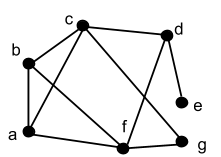
\includegraphics[width=4in]{Figure9}
			} \\\\
			{\color{blue} {\bf Figure 9:} \emph{An undirected graph has 7 vertices, a through g. There are 10-line segments that are between the following vertices: a and b, a and c, a and f, b and c, b and f, c and d, c and g, d and e, d and f, f and g. } }
			\\\\
			%Enter your answer below this comment line.
			All vertices have an even degree except for vertices 'c' and 'f', which
			have an odd degree.

			Therefore, it does not have an Euler circuit but has an Euler trail. An
			example of an Euler trail in this graph could be: $c \rightarrow a \rightarrow
			b \rightarrow c \rightarrow d \rightarrow e \rightarrow d \rightarrow f \rightarrow
			b \rightarrow f \rightarrow g \rightarrow c$. \\\\
	\end{enumerate}
	\newpage
	~\\
	\section*{Problem 5}
	Use Prim's algorithm to compute the minimum spanning tree for the weighted
	graph. Start the algorithm at vertex A. Explain and justify each step as you
	add an edge to the tree. \\
	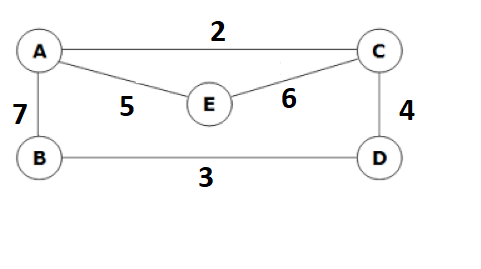
\includegraphics[width=5in]{prim}
	\\\\
	{\color{blue} {\bf Figure 10:} \emph{A weighted graph shows 5 vertices, represented by circles, and 6 edges, represented by line segments. Vertices A, B, C, and D are placed at the corners of a rectangle, whereas vertex E is at the center of the rectangle. The edges, A B, B D, A C, C D, A E, and E C, have the weights, 7, 3, 2, 4, 5, and 6, respectively. } }
	\\\\
	%Enter your answer below this comment line.
	\item \textbf{Start at vertex A}: It's the starting point of the algorithm.
	\item \textbf{Add the smallest edge connected to A}: The smallest edge is A-C
	with a weight of 2. I added this edge to the MST. \item \textbf{Consider all
	edges connected to the MST}: Next I noted edges A-E (5), A-B (7), C-D (4), and
	C-E (6). \item \textbf{Add the smallest edge not yet in the MST}: The smallest
	edge is C-D with a weight of 4. Add C-D to the MST. \item \textbf{Consider new
	edges connected to the MST}: Now I noted edges A-E, A-B, and E-C since D has
	no other connections not already in the MST. \item \textbf{Add the smallest
	edge not yet in the MST}: The smallest edge is A-E with a weight of 5. Add A-E
	to the MST. \item \textbf{Consider new edges connected to the MST}: Now I
	noted the edges A-B and E-C. \item \textbf{Add the smallest edge not yet in
	the MST}: The smallest edge is E-C with a weight of 6. None the less, an
	important note was how adding E-C would create a cycle, which is not allowed in
	a MST. Therefore, I essentially skipped this edge. \item \textbf{Add the
	smallest edge not yet in the MST}: The smallest remaining edge was A-B with a
	weight of 7. Add A-B to the MST.\\\\

	At this point, all vertices are included in the MST, and I ensured not to
	create any cycles. The edges included in the MST are A-C, C-D, A-E, and A-B, with
	total weights of 2 + 4 + 5 + 7 = 18.

	The minimum spanning tree using Prim's algorithm from vertex A is thus made up
	of the edges with weights 2, 4, 5, and 7.

	\newpage
	~\\
	\section*{Problem 6}
	A lake initially contains 1000 fish. Suppose that in the absence of predators
	or other causes of removal, the fish population increases by 10\% each month. However,
	factoring in all causes, 80 fish are lost each month.\\

	Give a recurrence relation for the population of fish after $n$ months. How many
	fish are there after 5 months? If your fish model predicts a non-integer
	number of fish, round down to the next lower integer. \\\\
	%Enter your answer below this comment line.
	The recurrence relation for the population of fish after $n$ months is given by:
	\[
		P(n) = P(n-1) \times 1.10 - 80
	\]
	with the initial condition being $P(0) = 1000$.

	This means that after 5 months, the fish population is predicted to be 1122 fish;
	rounding down to the nearest integer. \\\\
\end{document}